%! TEX program = xelatex
\documentclass[letterpaper,11pt]{article}

\usepackage[letterpaper,left=0.55in,right=0.55in,top=0.38in,bottom=0.45in]{geometry}
\usepackage{xcolor}
\usepackage{graphicx}
\usepackage{hyperref}
\usepackage{enumitem}
\usepackage{titlesec}

\hypersetup{%
  colorlinks=true,
  urlcolor=black,
  linkcolor=black
}

\pagestyle{empty}
\setlength{\parindent}{0pt}
\setlength{\parskip}{0pt}
\setlist[itemize]{leftmargin=0.28in,itemsep=0.25em,topsep=0.15em}
\sloppy

\titleformat{\section}
  {\large\bfseries\uppercase}
  {}
  {0pt}
  {}
  [\titlerule]
\titlespacing*{\section}{0pt}{0.78em}{0.28em}

\newcommand{\resumeHeader}[6]{%
  \noindent
  \begin{minipage}[c]{0.15\textwidth}
    \mbox{}
  \end{minipage}%
  \begin{minipage}[c]{0.70\textwidth}
    \centering
    {\LARGE\bfseries #1}\\[0.28em]
    #2\\[0.18em]
    {\small #3 $\diamond$ #4 $\diamond$ #5 $\diamond$ #6}
  \end{minipage}%
  \begin{minipage}[c]{0.15\textwidth}
    \raggedleft
    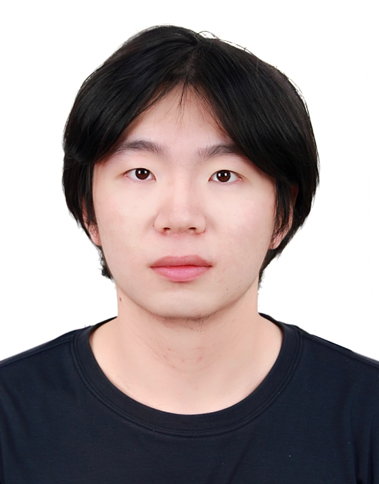
\includegraphics[width=0.95in,height=1.20in,keepaspectratio]{pic/cy.jpeg}
  \end{minipage}
  \vspace{0.42em}
}

\newcommand{\educationEntry}[3]{%
  \noindent
  \begin{tabular*}{\textwidth}{@{}p{0.76\textwidth}@{\extracolsep{\fill}}r@{}}
    #1, #2 & #3 \\
  \end{tabular*}
  \vspace{0.68em}
}

\newcommand{\skillLine}[2]{%
  \textbf{#1.} #2\par\vspace{0.32em}
}

\newcommand{\projectEntry}[2]{%
  \textbf{#1.} #2\par\vspace{0.62em}
}

\newcommand{\workExperienceEntry}[5]{%
  \noindent
  \begin{tabular*}{\textwidth}{@{}p{0.78\textwidth}@{\extracolsep{\fill}}r@{}}
    \textbf{#1} & \textbf{#4} \\
    \textit{#2} \enspace $\vert$ \enspace \textit{#3} & \\
  \end{tabular*}
  \vspace{-0.18em}
  \begin{itemize}[leftmargin=0.22in,topsep=0.12em,itemsep=0pt]
    \item #5
  \end{itemize}
  \vspace{0.18em}
}

\newcommand{\headerLink}[2]{%
  \href{#1}{\textcolor{blue}{\underline{#2}}}%
}

\begin{document}

\resumeHeader{YE CHENG}
  {080-4243-4567 $\diamond$ Kyoto, Japan} % chktex 8
  {\headerLink{mailto:teiyou416@gmail.com}{Mail}}
  {\headerLink{https://teiyou416.github.io}{Homepage}}
  {\headerLink{https://www.linkedin.com/in/ye-cheng-158360361/}{LinkedIn}}
  {\headerLink{https://github.com/teiyou416}{GitHub}}

\section{Education}

\educationEntry{\textbf{Master of Informatics}}
  {Kyoto University, Graduate School of Informatics}
  {2026.4 \textendash{} Expected 2028.3}

\educationEntry{\textbf{Bachelor of Engineering}}
  {Kansai University, Department of Civil, Environmental and Applied Systems Engineering}
  {2021.4 \textendash{} 2026.3}

\section{Skills}

\skillLine{Completed Course}{Data Structures and Algorithms, Operating Systems, Introduction to Artificial Intelligence, Computer Networks, Information Security,
Information Theory, Database Systems and so on}

\skillLine{Programming Skills}{Python, Golang, C, Vimscript, SQL, Rust}
\skillLine{Tools and Frameworks}{Node.js, Git, Linux, PyTorch, Docker, Vim, PostgreSQL, k8s}

\skillLine{Language Skills}{English (TOEIC score: 880/990), Japanese (JLPT N1), Chinese (Native)}

\section{Work Experience}

\workExperienceEntry{Rakuten Group}
  {Application Engineer (Intern)}
  {RUNA Backend Team, Global Ad Division}
  {Aug 2026--Oct 2026}
  {Developed a chatbot for RUNA, Rakuten's advertising delivery platform,
  as a member of the backend team. Implemented a retrieval workflow that
  searches Rakuten's internal Confluence documentation and returns relevant
  information in response to user queries. Integrated MCP-based tools to
  handle requests requiring additional context or actions and help users
  resolve issues.}

\section{Projects}

\projectEntry{Mogu Mogu}{Designed the backend architecture and core APIs for
an AI-powered calendar that recommends meals from users' schedules, activity,
and dietary history. Implemented JWT authentication, profile and event
management, recommendation workflows, and validation middleware using Go,
Gin, GORM, and PostgreSQL.}

\projectEntry{Simblock\_go}{Reimplemented the SimBlock blockchain network
simulator in Go, including a discrete-event engine, network topology
processing, Proof-of-Work consensus, and asynchronous handling of Inv, Block,
and CmpctBlock messages. Added YAML configuration, shell-based workflows, and
integration tests.}

\projectEntry{Conference Paper}{Proposed GOFA, a gradient-oriented backdoor
attack on Vertical Federated Learning that constructs poisoned samples from
server-returned gradients and masks their original features with adversarial
perturbations. Evaluated the method on CIFAR-10 and UCI-HAR with PyTorch and
CUDA; accepted by ICECET 2026.}

\end{document}
